%%
%% This is file `sample-sigconf.tex',
%% generated with the docstrip utility.
%%
%% The original source files were:
%%
%% samples.dtx  (with options: `sigconf')
%% 
%% IMPORTANT NOTICE:
%% 
%% For the copyright see the source file.
%% 
%% Any modified versions of this file must be renamed
%% with new filenames distinct from sample-sigconf.tex.
%% 
%% For distribution of the original source see the terms
%% for copying and modification in the file samples.dtx.
%% 
%% This generated file may be distributed as long as the
%% original source files, as listed above, are part of the
%% same distribution. (The sources need not necessarily be
%% in the same archive or directory.)
%%
%% Commands for TeXCount
%TC:macro \cite [option:text,text]
%TC:macro \citep [option:text,text]
%TC:macro \citet [option:text,text]
%TC:envir table 0 1
%TC:envir table* 0 1
%TC:envir tabular [ignore] word
%TC:envir displaymath 0 word
%TC:envir math 0 word
%TC:envir comment 0 0
%%
%%

\PassOptionsToPackage{lstlisting,prologue,dvipsnames}{xcolor}
%% The first command in your LaTeX source must be the \documentclass command.
\documentclass[sigconf]{acmart}
%% NOTE that a single column version may be required for 
%% submission and peer review. This can be done by changing
%% the \doucmentclass[...]{acmart} in this template to 
%% \documentclass[manuscript,screen]{acmart}
%% 
%% To ensure 100% compatibility, please check the white list of
%% approved LaTeX packages to be used with the Master Article Template at
%% https://www.acm.org/publications/taps/whitelist-of-latex-packages 
%% before creating your document. The white list page provides 
%% information on how to submit additional LaTeX packages for 
%% review and adoption.
%% Fonts used in the template cannot be substituted; margin 
%% adjustments are not allowed.
%%
%%
%% \BibTeX command to typeset BibTeX logo in the docs
\AtBeginDocument{%
  \providecommand\BibTeX{{%
    \normalfont B\kern-0.5em{\scshape i\kern-0.25em b}\kern-0.8em\TeX}}}

%% Rights management information.  This information is sent to you
%% when you complete the rights form.  These commands have SAMPLE
%% values in them; it is your responsibility as an author to replace
%% the commands and values with those provided to you when you
%% complete the rights form.

%% These commands are for a PROCEEDINGS abstract or paper.
\acmConference[BuildSys '23]{Make sure to enter the correct
  conference title from your rights confirmation emai}{November,
  2023}{Istanbul, Turkey}
%
%  Uncomment \acmBooktitle if th title of the proceedings is different
%  from ``Proceedings of ...''!
%
%\acmBooktitle{Woodstock '18: ACM Symposium on Neural Gaze Detection,
%  June 03--05, 2018, Woodstock, NY} 
%\acmPrice{15.00}
%\acmISBN{978-1-4503-XXXX-X/18/06}


%%
%% Submission ID.
%% Use this when submitting an article to a sponsored event. You'll
%% receive a unique submission ID from the organizers
%% of the event, and this ID should be used as the parameter to this command.
%%\acmSubmissionID{123-A56-BU3}

%%
%% For managing citations, it is recommended to use bibliography
%% files in BibTeX format.
%%
%% You can then either use BibTeX with the ACM-Reference-Format style,
%% or BibLaTeX with the acmnumeric or acmauthoryear sytles, that include
%% support for advanced citation of software artefact from the
%% biblatex-software package, also separately available on CTAN.
%%
%% Look at the sample-*-biblatex.tex files for templates showcasing
%% the biblatex styles.
%%

%%
%% The majority of ACM publications use numbered citations and
%% references.  The command \citestyle{authoryear} switches to the
%% "author year" style.
%%
%% If you are preparing content for an event
%% sponsored by ACM SIGGRAPH, you must use the "author year" style of
%% citations and references.
%% Uncommenting
%% the next command will enable that style.
%%\citestyle{acmauthoryear}

\usepackage[dvipsnames]{xcolor} % https://en.wikibooks.org/wiki/LaTeX/Colors
\definecolor{LightGray}{rgb}{0.97,0.97,0.97}
\usepackage{hyperref}
\usepackage{listings}
\usepackage{amsmath}
\usepackage{lipsum}
\usepackage{graphics}
\usepackage{array}


%%

\lstdefinelanguage{SPARQL}{
  basicstyle=\small\ttfamily,
  backgroundcolor=\color{LightGray},
  columns=fullflexible,
  breaklines=false,
  sensitive=true,
  % --------------------------
  frame=bt,
  aboveskip=1em,
  belowskip=1em,
  xleftmargin=.5em,
  xrightmargin=.5em,
  framexleftmargin=.5em,
  framextopmargin=.5em,
  framexbottommargin=.5em,
  framexrightmargin=.5em,
  % --------------------------
  tabsize = 2,
  showstringspaces=false,
  morecomment=[l][\color{gray}]{\#},       % comments
  morecomment=[n][\color{blue}]{<http}{>}, % uris
  morestring=[b][\color{OliveGreen}]{\"},  % strings
  % -------------------------- variables
  keywordsprefix=?,
  classoffset=0,
  keywordstyle=\color{Sepia},
  morekeywords={},
  % -------------------------- prefixes
  classoffset=1,
  keywordstyle=\color{Purple},
  morekeywords={rdf,rdfs,owl,xsd,purl,elem,tso,brk,hvac},
  % -------------------------- keywords
  classoffset=2,
  keywordstyle=\color{MidnightBlue},
  morekeywords={
    SELECT,CONSTRUCT,DESCRIBE,ASK,WHERE,FROM,NAMED,PREFIX,BASE,OPTIONAL,
    FILTER,GRAPH,LIMIT,OFFSET,SERVICE,UNION,EXISTS,NOT,BINDINGS,MINUS,a
  }
}
%% end of the preamble, start of the body of the document source.
\begin{document}

%%
%% The "title" command has an optional parameter,
%% allowing the author to define a "short title" to be used in page headers.
\title{Reasoning about Physical Processes in Buildings\\through Component Stereotypes}

%%
%% The "author" command and its associated commands are used to define
%% the authors and their affiliations.
%% Of note is the shared affiliation of the first two authors, and the
%% "authornote" and "authornotemark" commands
%% used to denote shared contribution to the research.
\author{Ganesh Ramanathan}
\email{ganesh.ramanathan@siemens.com}
\orcid{1234-5678-9012}
\affiliation{%
  \institution{Siemens AG}
  \country{Switzerland}
}
\author{Simon Mayer}
\email{simon.mayer@unisg.ch}
\orcid{0000-0001-6367-3454}
\affiliation{%
  \institution{University of St. Gallen}
  \country{Switzerland}
}

%%
%% By default, the full list of authors will be used in the page
%% headers. Often, this list is too long, and will overlap
%% other information printed in the page headers. This command allows
%% the author to define a more concise list
%% of authors' names for this purpose.
\renewcommand{\shortauthors}{Ramanathan and Mayer}

%%
%% The abstract is a short summary of the work to be presented in the
%% article.
\begin{abstract}
Buildings employ an ensemble of technical systems like those for heating and ventilation and each of them orchestrate complex physical processes.
%
Ontologies such as Brick, IFC, SSN/SOSA, and SAREF have been created to describe the technical systems in a machine-understandable manner.
%
However, such ontologies focus largely on describing system \emph{topology}, whereas several use cases, such as automated fault detection and diagnostics (AFDD), also need knowledge about the physical processes.
%
Physical processes can be described using mathematical simulation models, but this is practically too expensive for building automation systems and their integration with mainstream technical systems ontologies is still under-explored.
%
We propose to address these challenges by introducing the concept of \textit{component stereotypes} that describe the effect of component actuation on the state its underlying physical mechanism.
%
These stereotypes are then linked to actual component instances in the technical system description, thereby accomplishing an integration of structural description with knowledge about physical processes.
%
We contribute an ontology for such stereotypes and evaluate it with respect to the coverage of HVAC components in Brick and its ability to automatically infer relationships between components in a real-world building.
%
We show how the resulting knowledge graph can be queried by AFDD applications to know about expected consequences of an action, or conversely, identify components that may be responsible for an observed state of the process.
%
While we are able to report a coverage of 100\% of Brick HVAC components, the automatic inference underreports component dependencies in real-world installations. This points at a group of concepts which we propose should be considered in future versions of the Brick ontology.
%

\end{abstract}

%%
%% The code below is generated by the tool at http://dl.acm.org/ccs.cfm.
%% Please copy and paste the code instead of the example below.
%%

\maketitle
\section{Introduction}

Technical systems in a building are complex compositions of sub-systems and their components that work in tandem to carry out physical processes like heating, ventilation, and air-conditioning.
Traditionally, such systems were described in human-understandable ways like texts and diagrams; however, driven by the need to make such system knowledge more directly accessible to software applications, we are seeing more and more machine-understandable specifications in recent years.

A large part of this development builds on top of active and cross-cutting research in the engineering and Semantic Web communities, where several ontologies like Brick\footnote{\url{https://brickschema.org/ontology/}}~\cite{sd_balaji2016brick}, IFC\footnote{\url{https://technical.buildingsmart.org/standards/ifc/ifc-formats/ifcowl/}}~\cite{sd_ifc_beetz2009ifcowl}, SSN/SOSA\footnote{\url{https://www.w3.org/TR/vocab-ssn/}}, SAREF\footnote{\url{https://saref.etsi.org/core/v3.1.1/}}, etc. have made it possible to describe buildings and their systems in a manner that permits the creation of interoperable software on top of this knowledge~\cite{mayer2017open}.

Today, system design ontologies are used in the building automation domain to describe systems as compositions of sub-systems which are topologically related.
For example, using the Brick ontology, we can describe a heating system as a composition of sub-systems for heat generation, distribution, etc., each consisting of interconnected components like pumps, valves, etc.
In such models, \textit{components} (sometimes called \textit{equipment}) are the functional units that carry out a well-defined transformation of substance or energy.
Finally, the granularity of the decomposition of systems using these abstractions---systems, sub-systems, and components---varies from scenario to scenario and depends on the granularity and abstraction level at which it is desired to describe a system.
For example, a fan together with its motor and drive might be considered as a single \emph{component} when viewed from the perspective of a control program since this program is defined in terms of ``controlling the speed of the fan'' instead of adopting a more sub-system viewpoint (e.g., ``actuating the drive which controls the speed of the motor and consequently the speed of the impeller of the fan'').

%The principal concepts in these ontologies include the notion of \textit{systems} (e.g., heating, ventilation, lighting, etc.) which are designed to serve different requirements. Complex systems may be described in parts as \textit{sub-systems} which manage a distinct physical process (e.g., heating system comprising of heat generation, distribution, and terminal sub-systems). 
%Such components may be inter-connected (through relationships like "A \textit{feeds} B" etc.) so that the integrated physical process is reflected across the components.
In addition to the structural relationships between sub-systems and components, it is often desired to also encode knowledge about \textit{how the system functions}.
We see this need in several existing use cases like automated fault detection and diagnosis (AFDD; see~\cite{ramanathan2021assisting}), plausibility checking~\cite{gwerder2022data}, or control optimization~\cite{delgoshaei2017towards}.
Such knowledge further enables matching automation program strategies to system deployments, synthesizing control interlocks~\cite{koziolek2020industrial}, and may support autonomous software agents to control and coordinate a building automation system~\cite{ramanathan2021autonomous}.
%
For this purpose, we argue that machine-understandable system descriptions should not only incorporate structural descriptions, but also a description of the functioning of the system's components and the effects they have on observable physical states of the system's context.
%
For example, although we know that the supply fan of the Air Handling Unit (AHU) shown in Figure~\ref{fig:example-ahu} is an instance of Brick class \texttt{Supply\_Fan}, one has to rely on textual descriptions to understand that it functions by transferring kinetic energy from the impeller to the air resulting in increased air pressure and flow.
%
In a system like the AHU, for a software agent to answer the question ``Which components and which of their actions influence the supply air temperature?'', it would require access to common knowledge (in machine-understandable form) of the physical mechanisms each component of the AHU is involved in.

\begin{figure}[t]
\centering
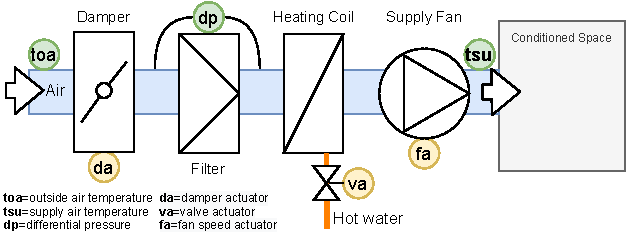
\includegraphics[width=0.9\linewidth]{figures/i_example_ahu.pdf}
\caption{An example of a system: This AHU takes in fresh air and filters and heats it before supplying it to a room. The value of \texttt{tsu} in this example is determined by \texttt{toa}, \texttt{da}, \texttt{va}, and \texttt{fa}.}
\vspace{-5mm}
\label{fig:example-ahu}
\end{figure}


%As an example, consider the Air Handling Unit (AHU) shown in Figure~\ref{fig:example-ahu}, which we will use as the running example in this paper.
%Ontologies like Brick provide taxonomies to describe the components of such a system in terms of the class hierarchy to which they belong along with properties to model relationships to other entities.
%However, such taxonomical and structural descriptions are insufficient to obtain a \textit{behavioral view} of the component.
%Consequently, though we have machine-understandable structural knowledge of systems, for example modeled using the Brick ontology\footnote{See \url{http://w3id.org/elementary/examples} for a model of the AHU}, answering a question like ``which components and which of their actions influence the supply air temperature?'' would require access to common knowledge (in machine-understandable form) of the physical processes that the AHU is involved in.

Traditionally, physical mechanisms are described using semi-formal diagrams, formal mathematical equations, logical rules, state machines, or simulation models.
%Ontologies such as OntoCape~\cite{morbach2009ontocape} and PhySys~\cite{borst1995physsys} enable modeling of physical processes in machine-understandable forms.
However, creating such models for systems deployed in buildings is prohibitively expensive due to the effort involved in modeling the mechanisms and their mathematical equations.
On the other hand, amongst the use cases which can benefit from the knowledge of physical mechanisms and processes, several of them, like AFDD, fault-mode-effect analysis, plausibility checking, and reasoning about control functions, do not require full simulation models, but would already benefit from more abstract knowledge in terms of dependencies between variables that represent the process mechanism.
%
Such information would informally read like ``The supply temperature is determined by the airflow rate (influenced by the fan and the damper), the energy input to the heating coil (influenced by water temperature and the flow rate determined by the valve), and the intake air temperature (which is not under system control)'' -- this would permit a human to for instance understand that too low supply temperature could be remedied by modulating the damper actuator, supply fan speed actuator, or the valve actuator of the heating coil.
Such a rule could further make explicit (or integrate) more fundamental knowledge (e.g., that the heating coil is the component that most directly influences supply air temperature).
Such knowledge can be further generalized by simplifying the description of the underlying physical mechanism: heating coils use the same physical mechanism as economizers or condensers---on this abstraction level, we may hence refer to all of these types of components as \emph{heat exchangers}.

%However, it is noticeable that the knowledge about the role of the components in the physical process is closely tied to the configuration of the technical system.
%For example, if the AHU were to have a second heating coil or have a mixed air inlet then the above stated rule has to be modified.
%Creating such a repertoire of functional descriptions is cumbersome because of the large combination of physical states and possible configuration of the technical systems.
%It is clear to us that a full-fledged physics model can not only take into consideration the current state of the process, but also consider the system dynamics in inferring the relationships.

Towards permitting practically feasible functional description of components, we formulate the following questions:
\begin{enumerate}
    \item How can we describe physical mechanisms in a simplified abstraction that is widely valid for components of a kind? 
    \item How can we link such (simplified) descriptions of a component's mechanism to its technical interfaces so that we can understand which interfaces are relevant in the functioning? 
    \item How can we enable reasoning about the role of components that are interlinked in a process?
\end{enumerate}


Our aim is hence to capture such common knowledge of physical processes in a building automation system and thereby enable the automated answering of queries about a system's overall behavior by permitting software programs (e.g., AFDD) to use formal reasoning on top of this knowledge. 
%
To do this, we propose a method to create \textit{stereotypical} behavioral descriptions of \textit{physical mechanisms} like \textit{heat exchange} or \textit{pressurization}.
The stereotype would describe the process variables and their inter-relationship in a high-level abstraction instead of a complete mathematical equation.
Such a fundamental description may be referred to and, hence, reused by various component kinds -- for example, the mechanism of \textit{heat exchange} is used by heating/cooling coils, evaporators, condensers, etc. in HVAC systems.
Further, in order to couple a component kind to the description of the physical mechanism(s) it uses, we propose a method to create \textit{stereotypical} descriptions of its \textit{technical interfaces} and couple them to the variables of the physical mechanism -- for example, the heating coil in the AHU has inlet and outlet ports for air and hot water. The temperatures and flow rates observed or effected at these ports can be related to the variables involved in the description of the heat exchange mechanism that the heating coil uses.
%
We contribute the concept of such \emph{stereotypes} and position it with respect to related work (see Section~\ref{sec:relwork}); we then provide the concepts and relationships required to model stereotypes of physical mechanisms and technical interfaces of system components (see Section~\ref{sec:approach}). The required concepts and relationships are provided in an ontology, which we name \emph{Elementary}\footnote{Inspired by the word often used by the popular detective character Sherlock Holmes.}. \emph{Elementary} is modeled using OWL, which is part of the Semantic Web technology stack, and widely used to create formal specification of concepts and relationships.
%
In Section~\ref{sec:evaluation}, we demonstrate the integration of our stereotypes with structurally oriented concepts of system components from the Brick ontology. This shows how structural knowledge can be combined with functional knowledge about the system components, and we illustrate the usage of our ontology by providing several examples of stereotypes along with a complete mapping of Brick HVAC components to proposed stereotypes.
%
Finally, we also provide an evaluation of our approach in a real setting of an office building that consists of about 180 rooms across six floors: We identified kinds of systems in the building that represent different levels of complexities in terms of topology and processes. We then identified kinds of queries found in AFDD use cases and show that our approach enables these to be answered without resorting to the use of full-fledged physics models.

%Therefore, by coupling the ports to the respective variables, we can create a machine-understandable description which can be used to infer that changing the flow rate or temperature of water at the inlet port will cause the outlet air temperature to be affected (note that employing a mathematical equation here could have established the tendency as increase in flow rate will cause rise in air outlet temperature).



%Such a stereotype describe how a typical instance of a component kind \textit{physical mechanisms} carried out by different component kinds.
%Such stereotypes correlate physical \textit{process variables} with one another, and further, to input, output, and actuation terminals of the component.
%The correlation is solely stated by identifying dependent and independent variables without involving a mathematical equation, and therefore cannot be used to predict dynamic or static values of the variables (hence our work is emphasised with the phrase \textit{naive stereotypes}).
%However, where available, the stereotypes can also be linked to mathematical or simulation models which can elucidate static and dynamic behaviour.
%The underlying stereotype of the physical mechanism helps us to infer the process role of a component based on its topological relationships (e.g., with \textit{feeds}) to other components.
%For example, if a fan feeds a heating coil then we can infer that the speed of the fan is one of the determining factors for the amount of thermal energy exchanged in the heating coil.

%\section{Related Work}
\section{Related Work}
\label{sec:relwork}

In most domains, systems engineering involves design of a system through decomposition of requirements to find functional abstractions, which are then organized into a hierarchy of sub-systems (see~\cite{sd_nielsen2015systems} for an in-depth treatment of this topic).
%Since standards for describing terms and relationships are common in engineering design~\cite{sd_yang2019ontology}, it was an almost natural step for practitioners to reuse these to create ontologies using Semantic Web technologies.
Ontologies such as Brick, IFC, SSN/SOSA, SAREF, etc. can be used to describe the sub-systems, their components, and interdependencies (e.g., in~\cite{sd_pauen2021tubes}).
Such ontologies model one or more of the following key aspects of structural descriptions in systems engineering~\cite{sd_van2013ontology,pp_borst1995physsys}: 
\begin{enumerate}
    \item The mereological (compositional) relationships in terms of sub-systems and components. For example, an AHU \textit{consists} of a heating coil, which in turn, has a control valve.
    \item The topological relationships (i.e., the physical process relationship between mereological entities. For example, using the Brick ontology, one can state that a \texttt{brick:Ra\-di\-a\-tion\_Hot\_Water\_System} consists of a number of instances of \texttt{brick:Ra\-di\-a\-tor}s which are of type \texttt{brick:Heat\_Ex\-chan\-ger} are placed in Rooms, and these are fed by an instance of a \texttt{brick:Boiler}.
    \item The domain-specific taxonomy to convey the \textit{functional abstraction} of a component (see~\cite{sd_yang2019ontology} for an extensive survey). For example, the class \texttt{brick:Fan} intends to describe all things that function like a \textit{stereotypical} fan. 
\end{enumerate}

While ontologies such as Brick capture a component's functional abstraction and integrate this with mereological and topological relationships, they do not seek to describe the \emph{physical manifestation of the behavior of a component}, which is what we claim to be required to answer the questions posed in the introduction. We hence seek to further integrate (in a way that is compatible with Brick and other widely used ontologies) knowledge about relevant aspects of this stereotypical behavior. We acknowledge (and support) that this knowledge might be further integrated with full simulation models of a component (e.g., towards realizing verifiably safe cyber-physical systems, see~\cite{pp_hybrid_tds_garcia2019hyplc}); however, we propose that an abstraction on the level of functional \emph{stereotypes} permits the automated query-answering across a broad range of relevant topics (such as AFDD) while remaining simple enough to be deployed in typical building automation systems.

Physical processes are typically described as sequences of \textit{physical mechanisms}, each of which is managed by a component in the system~\cite{pp_borst1995physsys,sd_akkermans1996ontology}.
%
% TSO, OntoCape, and PhySys need to be introduced somewhere here!!
Several ontologies (such as OntoCape~\cite{morbach2009ontocape}, TSO~\cite{sd_pauen2021tubes}, and PhysSys~\cite{borst1995physsys}) have been created for the purpose of describing physical processes and mechanisms.
These ontologies, which are grounded in standard physics and engineering knowledge, principally define a \textit{physical process} as a series of \textit{physical mechanisms} involving the transformation of energy, substance, or work.
According to Borst~\cite{borst1995physsys, sd_borst1997engineering}, these transformees are referred to as physical \textit{stuff}, and the transition of \textit{stuff} between process mechanisms is referred to as \textit{flow}.
Examples of such \textit{flow} of \textit{stuff} includes flow of air in a duct, electric current flowing in a wire, heat through a conductor, or force transmitted through a mechanical linkage.
Therefore, the term \textit{streams} or \textit{process pathways} is meant for describing and distinguishing the semantics of flow of stuff that occurs through a complex chain of components -- for example, \textit{supply}, \textit{extract}, etc.
%
To accomplish the automated inference of answers to questions such as those presented in the introduction, we hence require compatible ways of modeling the individual process mechanisms and of associating them with the respective technical components in a specific deployment.

The association of a technical component with a specific process mechanism is a commonality in these ontological approaches, which also stems from their origin in process and systems engineering theory.
Therefore, when components are connected to one another through their \textit{terminals} or \textit{ports}, their mechanisms are deemed to influence one another such that \textit{stuff} flows between them -- thereby creating a physical process; however, today, in building automation, neither the technical system description nor the physical process ontologies capture this coupling. 
% Ok, done with the linking part. Now we go to the modeling of individual process mechanisms.

Furthermore, our approach needs to provide a way of describing each process mechanism to convey knowledge about the transformation it performs. This is typically done using mathematical equations where the \emph{state} of the physical mechanism is represented using \textit{process variables} which are measurable quantities.
The behavior of individual mechanisms which are described using mathematical models (for example, using the EngMath~\cite{gruber1994ontology} ontology) can then be used by solvers to determine static and dynamic state changes in the process.
The mathematical models are constructed either from first principles of the physics involved or using \textit{system identification}, which is an approach where dynamical systems are observed and a model of their behavior is built using statistical methods.
However, creating such models for systems deployed in buildings is typically too expensive in practice due to the effort involved in modeling the mechanisms and their mathematical equations~\cite{wetter2019view}; this is due to models for real-life sub-systems often requiring extensive parameterization together with the computational effort required to simulate them.

On the other hand, engineering design primarily relies on considerably \emph{simplified} representations of these equations, which are presented in the form of tables and graphical plots in datasheets and design handbooks, and these are sometimes referred to as \textit{operational model}~\cite{pp_kief_yoshioka2004physical}.
For example, the datasheet of a centrifugal fan contains characteristic curves depicting the fan's operation under different conditions.
In addition to such information about a specific product's characteristics, an engineer has generalized heuristic knowledge about the physical principles involved -- for example, \textit{affinity laws} (see~\cite{stewart2018surface}) state the dependency between the speed of a fan impeller and the resulting flow rate.
At an even more abstract level of understanding, from such theory of widely applicable physical principles, one can recognize the independent and dependent variables involved in a physical mechanism.
Although such simplistic understanding is rarely sufficient when \emph{designing} a system, it does provide valuable knowledge to gain a high-level understanding of a deployed system's functioning.
For example, the knowledge that the speed of a fan's impeller determines the outlet flow rate, when coupled with structural knowledge that the fan feeds a heat exchanger and that a heat exchanger (stereotypically) has an inflow flow rate, serves to link the behavior of the fan to that of the heat exchanger.
An approach to model such an \textit{elementary} abstraction of the physical principles and their link to the technical components in a building automation system is today missing.
While in~\cite{hodges1995functional} understanding of simple mechanics is captured using an ontology, this limited to understanding human interactions with mechanical tools and does not address physical processes.

% But what is now missing here is why we don't use simulation models everywhere (effort; performance; etc.). This is especially important since your core argument in this paper is that both should (be there and should) be integrated. 
%A special case of static function is where the dependent variable has discrete states and therefore the process inputs can be considered as \textit{process actions} which cause state transitions.
%An action afforded by a component in the technical system acts on a physical mechanism through the change of an independent variable.
%For example, opening a radiator valve (component action) results in increased energy input (the independent variable) in the heat exchange mechanism of the heating process.
%However, currently, there is no bridging concept to link physical mechanisms to actions afforded in the technical system.
%As we shall see next, automation programs are designed against the affordances in the technical system.

We address this gap in our approach by modeling stereotypical knowledge about the physical mechanisms that a system component is involved in, and by integrating this knowledge in a way that is compatible with widely used ontologies for building automation components.
We claim that this enables the system to know enough about its functioning by allowing formal reasoning on top of this knowledge. This would, for example, enable automatically reasoning about the potential \textit{effects of an automation program} on the physical process, or to determine faults in the system that lead to unexpected functioning of a control program. The integration of mathematical models, which would permit deeper inspection of the system's behavior (at higher cost), remains possible with our approach.



%========================================================================================================
\section{Approach: Component Stereotypes}
\label{sec:approach}

In the previous section, we pointed out that physical mechanisms can be described in a generalized manner by solely identifying their independent and dependent variables and their inter-relationships.
This already would offer valuable knowledge for several use cases which requires a high-level understanding of the system functions.
%
We also highlighted that ontologies for structural description of systems provide domain-specific taxonomies to classify components according to functional abstraction along with description of their interconnections in the system topology.
%
However, we argue that an approach to interlink structural descriptions and knowledge of physical mechanisms is missing -- i.e., an approach is required that goes beyond component classification and topological description to include knowledge of physical mechanisms such that we understand \textit{how} a \emph{system of interconnected components} functions. 

To address this, we introduce the idea of \textit{stereotypes} for components of technical systems.
%In comparison with purely taxonomical classes, a stereotype can be examined \emph{as if it were a real component}.
%
To illustrate our idea of a stereotype, let us consider the fan in our AHU example (Figure~\ref{fig:example-ahu}).
We can imagine a \textit{stereotypical fan} as having an air inlet and outlet, and a impeller shaft; these form the fan's technical interfaces.
We further know that a fan uses the \textit{pressurization} mechanism whereby the speed of the impeller (effected at the shaft) determines the air flow rate (observable at the air outlet and inlet).
%
Now, when presented with an actual instance of a fan, we may integrate this stereotypical knowledge to gain an insight into how this instance can be acted upon and how it would behave in response. We can further use this to investigate the relationships between the fan instance and other technical components in a system such as the AHU.

The idea of a \textit{component stereotype} which we put forward encompasses stereotypical knowledge of \textit{technical interfaces} provided by the component kind and the \textit{physical mechanism} such a component uses.
Since a physical mechanism (e.g., heat exchange) may be applicable to more than one component kind, our proposed approach allows description of physical mechanisms in a way that it can be reused by multiple component stereotypes.
%
The resulting component stereotype is also agnostic of the exact process context.
%in which a component is deployed -- i.e., it focuses on describing a generalized behavior of the component kind which, for example, domain experts and manufacturers can provide.
For example, the stereotype of the fan would be applicable irrespective of whether it is used for driving airflow for heat exchange or for ventilation.
In other words, a stereotype is a reusable artifact for the domain and is not specifically crafted for a particular instance of a component, a system, or the role a component plays in a system.
This supports practical applicability of our approach -- when supplied with a topological model of component instances, the only remaining task during engineering is to link these instances to suitable stereotypes.


\subsection{Elementary: An Ontology for Stereotyping}

We propose the \emph{Elementary} (prefix: \texttt{elem:}) ontology\footnote{Available at \url{http://w3id.org/elementary}} to support the creation of stereotypes and the interlinking with topology-oriented system descriptions such as in Brick.
%
\emph{Elementary} addresses three aspects involved in defining and using stereotypes: 1. A way to express physical mechanisms in terms of its relation to process variables, 2. a way to describe the process semantics of interfaces of the stereotypical components and link them to description of mechanisms, 3. support for automatic inference of the effect of interactions between the components on the process which they are part of. 

%If we reflect back on our example question about  "The supply temperature is determined by the air flow rate (influenced by the fan speed and the damper opening), the energy input (influenced by water temperature and the flow rate determined by the valve), and the intake air temperature". 

%The application of our approach involves two sub-tasks: As a first task, using our ontology, domain experts create libraries of (reusable) stereotypes of component's interfaces and their physical mechanisms. For example, a stereotype of a \texttt{centrifugal-fan} would state (mereologically/topologically) that it has air inlet and outlet ports and an and impeller shaft to which mechanical power can be supplied, while the associated stereotypical (functional) mechanism of pressurization would correlate air inlet pressure and shaft rotation speed to outlet flow rate.

%Such stereotypes are represented as individuals in RDF instead of using OWL class restrictions because formulation of SPARQL queries is more convenient and intuitive.

%In the second part, instances of components in a specific deployment of a system need to be linked to appropriate stereotypes. The individual component instances might be described already using a suitable ontology such as Brick. For example, for a recirculating AHU, the heating coil would be linked to the stereotype of \texttt{forced-flow-heat-exchanger} whereas both supply and extract fans would be linked to the stereotype of \texttt{centrifugal-fan}.

\begin{figure}[t]
\centering
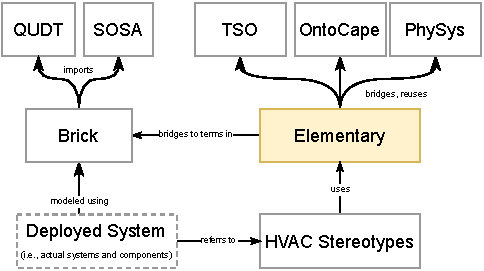
\includegraphics[width=6cm]{figures/a_overview_of_ontologies_involved.pdf}
\caption{The \emph{Elementary} ontology and its relation to other ontologies. Actual systems are modeled using Brick and each component instance in the system is linked to a stereotype in the domain-specific library of stereotypes for HVAC components.}
\label{fig:overview}
\end{figure}

\textit{Elementary} reuses terms and relationships from several openly available ontologies. An overview of \emph{Elementary} is shown in Figure~\ref{fig:overview}.
From TSO, OntoCape, and PhySys, we reuse concepts concerning physical processes, mechanisms, and flow of physical \textit{stuff}.
We bridge to Brick (which imports QUDT and SSN/SOSA) to reuse abstract concepts related to system design, and concrete instances depicting substance and quantities.
Further, to evaluate our approach, we have created a library of stereotypes for HVAC component kinds (prefix: \texttt{hvac}) that are available in the Brick ontology.
The actual systems that we used for our evaluation (see Section~\ref{sec:evaluation}) are modeled using the Brick ontology and are linked to stereotypes in this library.
%-----------------------candidate for removal-----------------------
The following snippet in RDF shows how two of the components of our AHU example that are modeled using Brick can be linked to their corresponding stereotypes:

\begin{lstlisting}[language=SPARQL]
urn:fan_01 a brick:Fan;
urn:fan_01 brick:feeds urn:heating_coil_01;
urn:fan_01 elem:hasStereotype hvac:centrifugal-fan.

urn:heating_coil_01 a brick:Hot_Water_Coil;
urn:heating_coil_01 elem:hasStereotype hvac:heat-exchanger.
\end{lstlisting}

In this snippet, we see two instances which are classified as \texttt{brick:Fan} and \texttt{brick:How\_Water\_Coil} and topologically linked using the \texttt{brick:feeds} relationship.
We will show how the stereotypes \texttt{hvac:cent\_rif\_ugal-fan} and \texttt{hvac:heat-ex\_chan\_ger} are created and how they lead us to infer the semantics of the process.
%------------------------------------------------------------------------

In the following sections, we describe in detail the three aspects behind our ontology, i.e. means of modeling stereotypes of physical mechanisms, coupling them to stereotypical component interfaces, and finally means of using the stereotypes to infer process relationships of actual components.
%What are components? Properties of a component that define its stereotype -- ports (connection points) and its semantics and physical mechanism. Problem of connecting components -- matching port semantics. Problem of feeds relationship not necessarily following process sequence -- idea of streams. Linking actuators to components -- actuators indeed feed force or energy.

\begin{figure}[t]
\centering
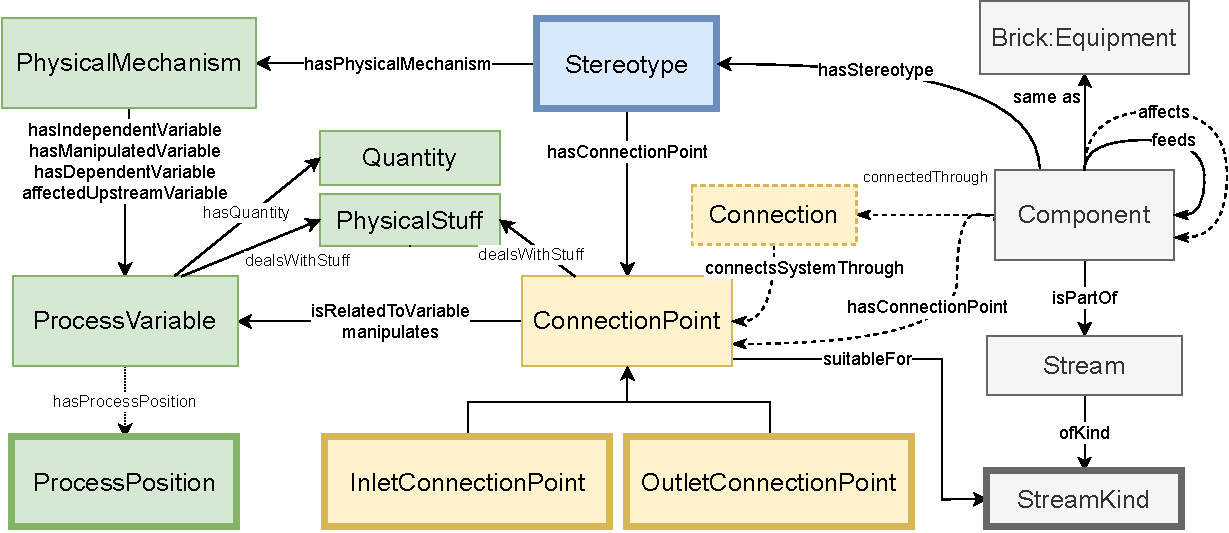
\includegraphics[width=8.5cm]{figures/a_overview_of_classes_in_elementary.pdf}
\caption{The principal classes of the \emph{Elementary} ontology. Boxes with thick border are classes which we have added while others are reused from existing ontologies. Dashed lines and borders indicate relationships and instances that are inferred.}

\label{fig:elementary-detailed-view}
\end{figure}


\subsection{Modeling Physical Mechanisms}

Mathematical models of physical mechanisms are typically expressed as equations which refer to \textit{process variables}.
More specifically, these are \textit{independent variables} (IV) and \textit{dependent variables} (DV) -- in the mathematical equation, IVs appear as parameters of a function whose output are one or several DVs.
In other words, by changing values of IVs, the effect of the mechanism can be observed as change of the DVs.
The variables are described by: 1. their \textit{position} with respect to the physical mechanism (e.g., at the inlet or outlet), 2. the \textit{physical stuff} whose state a variable represents, and 3. the \textit{quantity} the variable conveys (e.g., temperature, energy content, pressure, or force)~\cite{borst1995physsys,preisig2021ontology,cessenat2018mathematical}.
In the context of the AHU example, Figure~\ref{fig:process-variables} shows the process variables associated with the process mechanism of \emph{heat exchange}, i.e., the stereotypical mechanism used by the AHU's heating coil.
Here, $T_{aout}$ is a DV which is influenced by $Q_{a}$, $Q_{w}$, $T_{ain}$, and $T_{win}$ -- i.e. the IVs.
%\footnote{Note that though $T_{wout}$ appears in the steady-state equation for $T_{aout}$, it is not an IV, but in fact, is a DV}.
Though a number of IVs may influence a single DV, only a subset of them is meant to be \textit{manipulated}, i.e, changed by external action -- in controls engineering theory, such a variable is called a \textit{manipulated variable} (MV).
In the above example, $T_win$ are $Q_w$ are potential MVs.

Although most physical mechanisms that we encounter in building systems exhibit one-to-one relationships between MVs and DVs, there are several cases where a single MV influences more than one DVs (e.g., compression can cause decrease in volume and increase in temperature), or, vice-versa, where several MVs influence a single DV (e.g., in a heating coil where both flow rate and water inlet temperature influence the air temperature).
On the other hand, disjointness of MVs and affected DVs in a mechanism indicates the presence of two distinct underlying mechanisms~\cite{top1991computational} and thus motivates refactoring the model.
%
Our model needs to furthermore consider that a DV of a mechanism might also affect \emph{upstream} mechanisms -- for example, flow caused by a centrifugal pressurization mechanism in a fan results in a suction effect at the inlet port which might cause flow in upstream components.

\begin{figure}[t]
\centering
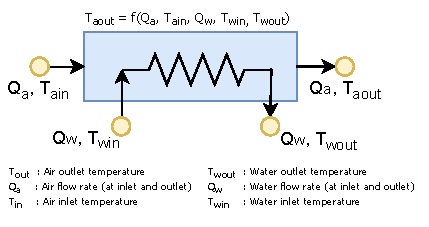
\includegraphics[width=0.9\linewidth]{figures/a_mpm_process_variables.pdf}
\caption{The stereotypical mechanism of heat exchange and its associated variables. The orange circles represent the terminals or ports of a component like heating coil which uses this mechanism.}
\label{fig:process-variables}
\end{figure}

We capture these concepts in the \emph{Elementary} ontology (see Figure~\ref{fig:elementary-detailed-view}) beginning with the class \texttt{elem:Process\-Variable} to describe a variable using relationships \texttt{elem:deals\-With\-Stuff}, \texttt{elem:has\-Pro\-cess\-Po\-si\-tion}, and \texttt{elem:has\-Quantity}.
Individuals of class \texttt{elem:Process\-Mech\-ani\-sm} are then related to one or more instances of \texttt{elem:Process\-Variable} through the relationships \texttt{elem:has\-In\-de\-pen\-dent\-Variable} (or its sub-type \texttt{elem:has\-Ma\-ni\-pu\-la\-tedVa\-ri\-a\-ble}) and \texttt{elem:has\-De\-pen\-dent\-Va\-ri\-a\-ble}.
Finally, to capture upstream effects of physical mechanisms, our model provides a transitive relationship \texttt{elem:aff\-ect\-ed\-Up\-str\-eam\-Var\-ia\-ble} between a physical mechanism and a DV.
%
Using these classes and relationships, one can define stereotypes of variables and mechanisms that are independent of the specific deployment context and, as we will describe in sub-section~\ref{subsec:process-relationship}, they can be interlinked with variables in other process mechanism stereotypes.
The following snippet of RDF/Turtle shows part of a stereotype for pressurization mechanism:

\begin{lstlisting}[language=SPARQL]
:pressurization rdf:type owl:NamedIndividual,
 elem:PhysicalMechanism ; 
 elem:hasIndependentVariable:inlet-air-pressure; 
 elem:hasDependentVariable:outlet-air-flow;
 elem:hasManipulatedVariable:shaft-speed;
# An example variable:
:oulet-air-flow rdf:type owl:NamedIndividual ,
 elem:ProcessVariable ;
 elem:dealsWithStuff brick:Air;
 elem:hasProcessPosition elem:outlet;
 elem:hasQuantity brick:Flow.
\end{lstlisting}

\subsection{Linking Components to Mechanisms}

The description of a general physical mechanism achieved in the step above allows us to query which IVs of a mechanism can be manipulated and the corresponding DVs that are influenced by these.
Next, we require a way that permits us to link ports (interfaces) of a component kind to the stereotype of the physical mechanism it uses. 
For example, heating coils, such as the one in the AHU, use the stereotypical heat exchange mechanism that we described as an example in the previous section.
Now, we need a way to infer which port (interface) of the heating coil is involved in manipulating the MV representing the water flow rate.
A domain expert would, in this case, know that this interface is the water inlet port, similar to the case of a fan, where an expert would know that mechanical force input at the shaft manipulates the fan speed.
Based on these observations, to enable the \emph{automatic} inference of such knowledge, we link the \emph{technical interfaces} of a component kind to the (stereotypical) process mechanism the component uses.
To model this relationship, we first require a way to describe \textit{stereotypical interfaces} expected in the components and then a way to link these to process variables associated with the corresponding mechanisms.

Several technical systems ontologies, such as OntoCape, PhysSys, and TSO already define the concept of a \textit{terminal}, \textit{connection point}, or \textit{port} to refer to a physical interface offered by the component through which flow of \textit{physical stuff} can be observed or effected~\cite{borst1995physsys,morbach2009ontocape,sd_pauen2021tubes}.
Such a \textit{connection point} is described in terms of the physical \textit{stuff} that flows through it together with the direction with respect to the component in which it flows (e.g., an ``air inlet'').
%I am removing this. It is a interesting and useful concept, but does not play a role in what we describe this paper.
%In addition, an \textit{action} is associated with the connection point to indicate the causation of the flow -- for example, air flow at the inlet of a heat exchanger is caused by a pressure difference; electrical current at a terminal is caused by a potential difference.
% https://www.w3.org/TR/2013/REC-prov-o-20130430/#wasInfluencedBy

To describe technical interfaces, our ontology reuses the class \texttt{tso:Con\_nect\_ion\_Point} to represent a terminal along with the relations \texttt{elem:dealsWithStuff} which links the terminal to individuals of \texttt{elem:Phy\-si\-cal\-Stuff}. These individuals could then, for instance, be of type \texttt{brick:Substance} or \texttt{tso:Energy}.
%Furthermore, the relation \texttt{elem:hasCausationAction} links to one of the individuals of type \texttt{elem:ActionType} (for example, \texttt{elem:pressure-drop}).
Since connection points are semantically qualified as inlet or outlet depending on the direction of the flow, we propose the sub-classes \texttt{elem:In\-let\--Conn\-ec\-tion\-Point} and \texttt{elem:Out\-let\-Conn\-ec\-tion\-Point}. 
\begin{figure}[t]
\centering
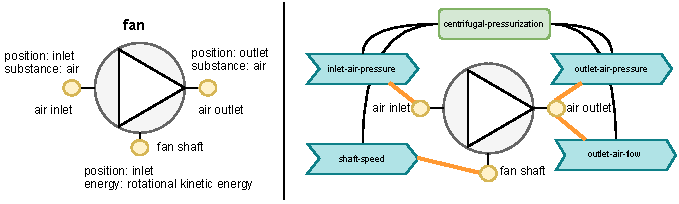
\includegraphics[width=8cm]{figures/a_lcm_variables_to_connections.pdf}
\caption{An example of a fan with its stereotypical physical mechanism, associated variables, and relation to the connection points.}
\label{fig:linking-connection-points-to-variables}
\end{figure}

Having created the means to specify process semantics for the connection points of a component, we now describe our approach to linking it to the stereotypes of the physical mechanism and variables we achieved in the previous step.

Considering the example of the fan in the left part of Figure~\ref{fig:linking-connection-points-to-variables}, a typical domain expert would be aware of these facts:

\begin{itemize}
    \item The fan uses the process mechanism stereotype of \texttt{cen\-tri\-fu\-gal press\-ur\-i\-za\-tion}; 
    \item the air pressure and volumetric flow can be observed at the inlet and outlet connection points; and
    \item the shaft of the fan's impeller (i.e., another connection point) can be supplied with torsional force to increase its speed.
\end{itemize}

This association is illustrated on the right side of Figure~\ref{fig:linking-connection-points-to-variables}.

The linking of the process variables to the corresponding connection points enables software agents to automatically infer that changing the  mechanical power input to  the impeller shaft will result in change in volumetric flow rate at the fan's air outlet.
Therefore, a component kind stereotype (like \texttt{hvac:centrifugal-fan}) should link the description of its typical technical interfaces to the description of a general physical mechanism (like \texttt{hvac:\-cen\-tri\-fug\-al-pr\-ess\-uri\-za\-ti\-on}) that is used by it.

To accomplish this, we provide the relationship \texttt{elem:is\-Re\-la\-ted\-To\-Va\-ri\-able} with \texttt{elem:Connection\-Point} as domain and \texttt{elem:Process\-Variable} as range.
In many cases, the designer of the component stereotype furthermore knows if an \texttt{elem:Conn\-ec\-tion\-Point} is meant to be used for manipulation of a process variable.
In such cases, the relationship should be specified using the property sub-type \texttt{elem:manipulates}. 
%

The following snippet shows an example of these relationships applied in the context of the definition of a stereotypical fan (in RDF/Turtle).

\begin{lstlisting}[language=SPARQL]
:centrifugal-fan rdf:type owl:NamedIndividual,
 elem:Stereotype ; 
 elem:hasConnectionPoint :cp_fan_air_inlet; 
 :cp_fan_air_outlet, :cp_fan_shaft;
 elem:hasProcessMechanism hvac:pressurization.

:cp_fan_air_outlet rdf:type owl:NamedIndividual ,
 elem:OutletConnectionPoint ;
 elem:dealsWithStuff brick:Air;
 elem:isRelatedToVariable hvac:inlet-air-pressure.

:cp_fan_shaft rdf:type owl:NamedIndividual ,
 elem:InletConnectionPoint ;
 elem:dealsWithStuff elem:mechanical_force;
 elem:manipulates hvac:shaft-speed.
\end{lstlisting}

Based on this example, the following SPARQL query shows how the relationship between the component's interfaces and the associated physical mechanism can be used to determine what inputs influence the airflow rate.
%Such queries are valuable for applications like AFDD which would have otherwise required off-band and installation-specific knowledge to be encoded in their program.

\begin{lstlisting}[language=SPARQL]
SELECT * WHERE {
 urn:fan_01 elem:hasStereotype ?s.
 ?s elem:hasProcessMechanism ?m.
 ?m elem:hasIndependentVariable ?iv.
 ?m elem:hasDependentVariable ?dv.
 ?dv elem:dealsWithStuff brick:Air. 
 ?dv elem:hasQuantity brick:Flow.
 ?s elem:hasConnectionPoint ?cp.
 ?cp elem:manipulates ?iv;
}
\end{lstlisting}
\vspace{-5mm}

%I think this is minor detail and should be skipped.
%Though it is possible to infer actions on connection points that can manipulate an independent variable (and consequently the dependent variable), in some component kinds only a sub-set of such connection points are meant to be used by an external agent.
%In such cases, explicit definitions of \texttt{elem:ComponentAction} can be used to adorn a component through \texttt{elem:hasComponentAction}. The \texttt{elem:ComponentAction} links the texttt{elem:ConnectionPoint} where the external agent can act.


\subsection{Inferring Process Relationships}
\label{subsec:process-relationship}
In this section, we explain how the stereotypes of the individual components which are interconnected in a system collectively help infer the \textit{process relationships}.
%
For example, in the AHU (Figure~\ref{fig:example-ahu}), increasing the air flow rate (by increasing the fan speed) affects the air outlet temperature of the heating coil (assuming constant energy input to the heating coil).
To infer this relationship, we require an approach that automatically links the DVs of one component to the IVs of other affected components.

Often topological descriptions of technical systems, like those based on Brick or IFC, do not model connection points of components (like for example in TSO) explicitly, but instead link the components with one another using a generic relationship such as \texttt{brick:feeds}.
On the one hand, using a generic relationship between components makes it easier to create system design descriptions, but on the other hand, it is not expressive enough when we want to understand the process relationships -- Figure~\ref{fig:feeds-is-insufficient} illustrates this situation.


\begin{figure}[t]
\centering
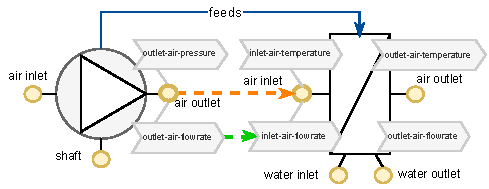
\includegraphics[width=0.9\linewidth]{figures/a_ipr_inter_connections.pdf}
\caption{Modeling a connection between two components (fan and heating coil) using a generic \texttt{feeds} relationship is insufficient to infer which specific connection points are connected (e.g., it is not specified whether the fan air outlet is connected to the heating coil's water inlet or its air inlet). However, by considering the characteristics of the connection points, inferences can be drawn about their relationship (orange dashed line), and further, about relationship between the variables (green dashed line).}
\label{fig:feeds-is-insufficient}
\vspace{-5mm}
\end{figure}


%---------- SHOULD THIS BE MOVED TO RELATED WORKS --------------------
%Before we present our proposed matching rule, we need to introduce an important concept in process engineering called \textit{Streams} or \textit{process pathways} are meant for describing and distinguishing the semantics of flow of stuff that occurs through a complex chain of components.
%In the example of the AHU, we have two streams involved: 1. The supply air stream which transports air from outdoor to the conditioned space with multiple physical mechanisms affecting the properties of the air that passes through, and 2. The hot water stream where thermal energy from the central heat generator is carried to the heating coil and circulated back (hence, often known as the \textit{hot-water circuit}).
%It is important to note that a stream may have flow of more than one physical stuff.

In a system scenario, components are parts of \textit{streams} (see Section~\ref{sec:relwork}): a concept which is essential in describing semantics of a connection point and process relationships between components.
For example, an AHU economizer has two air inlet connection points, one of which is meant for a \textit{fresh-air} stream, while the other is meant for an \textit{extract-air} stream.
In the HVAC domain, \emph{supply-air}, \emph{extract-air}, etc. are examples of well-known stream kinds.

Our ontology supports the integration of streams by providing a class \texttt{elem:Stream} and to permit assigning these to domain-specific \texttt{elem:StreamKind} (through the property \texttt{elem:has\-Stream\-Kind}).
Component instances may be assigned to one or more \texttt{elem:Stream}s through the \texttt{elem:isPartOf} relationship.
Similarly, a \texttt{elem:Con\-nen\-ctn\-ionn\-Pon\-int} may be specified to be suitable for a particular stream kind using the relationship \texttt{elem:suit\-able\-For}.

In order to infer connection between connection points described by the respective stereotypes of two components (in a \texttt{feeds} relationship), we match the following characteristics of the connection points:

\begin{enumerate}
    \item \emph{Matching Stream}: Both components should be part of the same \texttt{elem:Stream}
    \item \emph{Compatible Directionality}: Only an \texttt{elem:Outlet\-Con\-ne\-ct\-ion\-Poi\-nt} of the source component can connect to an \texttt{elem:In\-let\-Con\-ne\-ct\-ion\-Po\-int} of the target component.
    \item \emph{Compatible Stuff}: Both connection points should deal with the same (or compatible) physical \textit{stuff}.
    \item \emph{Matching StreamKind}: In case, multiple connection points of a component stereotype have the same attributes in terms of directionality and physical stuff, the \texttt{elem:StreamKind} of the connection points should match.
\end{enumerate}

For two \texttt{elem:Con\-n\-ec\-tin\-on\-Poi\-nts} which are inferred to be connected using this set of rules, the DV of the \texttt{elem:Ou\-tl\-etn\-Con\-ne\-ct\-ion\-nP\-ort} is consequently inferred to \text{elem:man\-ipun\-lates} the IV related to the \texttt{elem:In\-let\-Con\-nec\-tion\-Port} to which it connects.
If the downstream component has a DV which is an \texttt{elem:aff\-ec\-ted\-Up\-st\-re\-am\-Var\-ia\-ble} of the mechanism, then it is inferred to \text{elem:ma\-ni\-pu\-la\-te} the corresponding IVs on the upstream component.

We hence propose to infer process dependencies between actual components with the help of their respective stereotypes.
For example, using this approach we come to know that the outlet air temperature of an instance of a \texttt{brick:Heating\_Coil} is influenced by the connected instances of \texttt{brick:Fan} (influences air flow) and \texttt{brick:Heating\_Valve} (influences inlet water flow).
%, thereby enabling us to infer the effect of a process mechanism (used by a component) on both upstream and downstream parts of the system.
This enables both, automatically inferring potential influences of manipulation of a component interface on the system functioning (for e.g., in fault detection) and tracing potential causes of an observed effect to components and their interfaces (e.g, in fault diagnosis).

\section{Evaluation}
\label{sec:evaluation}

We report on two types of evaluations we have performed on our approach: 1. To examine the expressivity and generalizability (see Section~\ref{subsec:Expressivity}) and 2. to study its effectiveness when reasoning about the component's role in a process (see Section~\ref{subsec:Deployment}).

\subsection{Applying Stereotypes to Brick Components}
\label{subsec:Expressivity}

The use of the Brick ontology to model technical systems in real buildings has shown that its component classes are sufficient to cover common HVAC applications in buildings~\cite{sd_balaji2016brick}, and we use this result to demonstrate that our proposed approach can be used to describe the component stereotypes for these classes.
From the sub-classes of \texttt{brick:HVAC\_E\-quip\-ment}, we identified all classes that represent components -- i.e., those which use a distinct \textit{physical mechanism}.


%=======================================Table 1========================================================

\begin{table}[ht]
\small
\begin{tabular}{|l|l|l|}
\hline
   & \textbf{Brick Class} & \textbf{Mechanism Stereotype} \\ \hline
1  & Boiler               & heat-generation  \\ \hline
2 & Heat\_Exchanger      & heat-exchange     \\ \hline
3  & Cooling\_Tower       & heat-exchange    \\ \hline
4  & Economizer           & heat-exchange    \\ \hline
5  & Cold\_Deck           & heat-exchange   \\ \hline
6 & Radiator             & heat-exchange     \\ \hline
7  & Condenser            & heat-exchange    \\ \hline
8 & Space\_Heater        & radiative-heating \\ \hline
9 & Air\_Diffuser        & throttling        \\ \hline
10 & VAV                  & throttling       \\ \hline
11  & HVAC\_Valve          & throttling                      \\ \hline
12  & Damper               & throttling                      \\ \hline
13 & Isolation\_Valve     & throttling                      \\ \hline
14  & Bypass\_Valve        & throttling                      \\ \hline
15 & Fan                  & pressurization           \\ \hline
16 & Pump                 & pressurization           \\ \hline
17  & Compressor           & pressurization           \\ \hline
18 & Filter               & particulate-separation         \\ \hline
19 & Humidifier           & vapor-humidification            \\ \hline
20 & Motor                & electromagnetic-actuation     \\ \hline
\end{tabular}
\caption{Classes of components available in Brick and the proposed stereotype of the mechanism it employs.}
\label{tab:brick-mapping}
\vspace{-4mm}
\end{table}

%=======================================================================================================


After the identification of all such components\footnote{Some Brick classes like \texttt{brick:AHU} implement much more complex behavior than individual components; we consequently treat them as systems of components and they are hence not included in our stereotype matching table.} in the Brick ontology, we created stereotype definitions consisting of description of physical mechanisms and technical interfaces. This creation of stereotypes was done together with a HVAC domain expert, and we then related these definitions to the classes of components in Brick. Table~\ref{tab:brick-mapping} shows that our proposed stereotypes can be applied to all Brick components and can hence be used to describe what action can be taken on a component together with its physical effects.



%=========================================================================================
\begin{table*}[ht]
\small
\centering
\begin{tabular}{|l|l|l|l|l|}
\hline
\textbf{Mechanism Stereotype}         & \textbf{Input Interface} & \textbf{Manipulated Variable}                                                                    & \textbf{Affected Variable}                                                                                    & \textbf{Output Interface}                                                                 \\ \hline
heat-generation            & electrical-input             & electrical-power                                                                                 & water-outlet-temperature                                                                                      & water-outlet                                                                          \\ \hline
heat-exchange              & primary-fluid-inlet          & \begin{tabular}[c]{@{}l@{}}primary-fluid-flowrate\\ primary-fluid-inlet-temperature\end{tabular} & \begin{tabular}[c]{@{}l@{}}secondary-fluid-outlet-temperature\\ primary-fluid-outlet-temperature\end{tabular} & \begin{tabular}[c]{@{}l@{}}primary-fluid-outlet\\ secondary-fluid-outlet\end{tabular} \\ \hline
radiative-heating          & electrical-input             & electrical-power                                                                                 & air-temperature                                                                                               & conditioned-space                                                                     \\ \hline
throttling                 & actuation-input              & orifice-opening-ration                                                                           & \begin{tabular}[c]{@{}l@{}}fluid-flow-rate\\ fluid-outlet-pressure\end{tabular}                               & fluid-outlet                                                                          \\ \hline
fluid-pressurization       & shaft                        & mechanical-work                                                                                  & \begin{tabular}[c]{@{}l@{}}fluid-outlet-pressure\\ fluid-inlet-pressure\\ fluid-flow-rate\end{tabular}        & \begin{tabular}[c]{@{}l@{}}fluid-outlet\\ fluid-inlet\end{tabular}                    \\ \hline
particulate-separation     & none                         & none                                                                                             & fluid-outlet-particle-count                                                                                   & fluid-outlet                                                                          \\ \hline
vapor-humidification       & steam-inlet                  & steam-flowrate                                                                                   & air-outlet-humidity                                                                                           & air-outlet                                                                            \\ \hline
electro-magnetic-actuation & electrical-input             & electrical-power                                                                                 & mechanical-work                                                                                               & shaft                                                                                 \\ \hline
\end{tabular}
%=========================================================================================
\caption{Querying the stereotype mechanism description suggests which \emph{Input Interface} of the component (that uses the mechanism) can be acted upon towards affecting which \emph{Manipulated Variable}. It further links this manipulation to the \emph{Affected Variable} and gives the \emph{Output Interface} at which this effect can be observed.}
\label{tab:mechanisms-query}
\vspace{-4mm}
\end{table*}

For the stereotypes which we associated to the Brick classes, we then verified if it is possible to find out the relationships between the input interface, the process variable it manipulates, the process variable that will be affected, and the output interface of the component where the effect can be observed.

To evaluate this, we created a SPARQL query to run on the HVAC stereotypes ontology, and presented the results (see Table~\ref{tab:mechanisms-query}) to three HVAC domain experts.
The domain experts confirmed that our system's results were correct and sufficient to gain a high-level understanding of the IVs, MVs, and DVs in the components and to identify the connection points where the MVs can be manipulated.


\subsection{Understanding Processes using Stereotypes}
\label{subsec:Deployment}

To evaluate whether our approach is indeed sufficient to reason about a component's role in a real process, we examined the HVAC sub-systems in an office building consisting of about 180 rooms located across six floors which are served by central plants like AHUs, boilers, and chillers. 
%
From the system's engineering data available to us in this context, we chose the following system kinds (SK) in the order of increasing complexity (see Figure~\ref{fig:four-kinds-of-systems}):

\begin{figure*}[t]
\centering
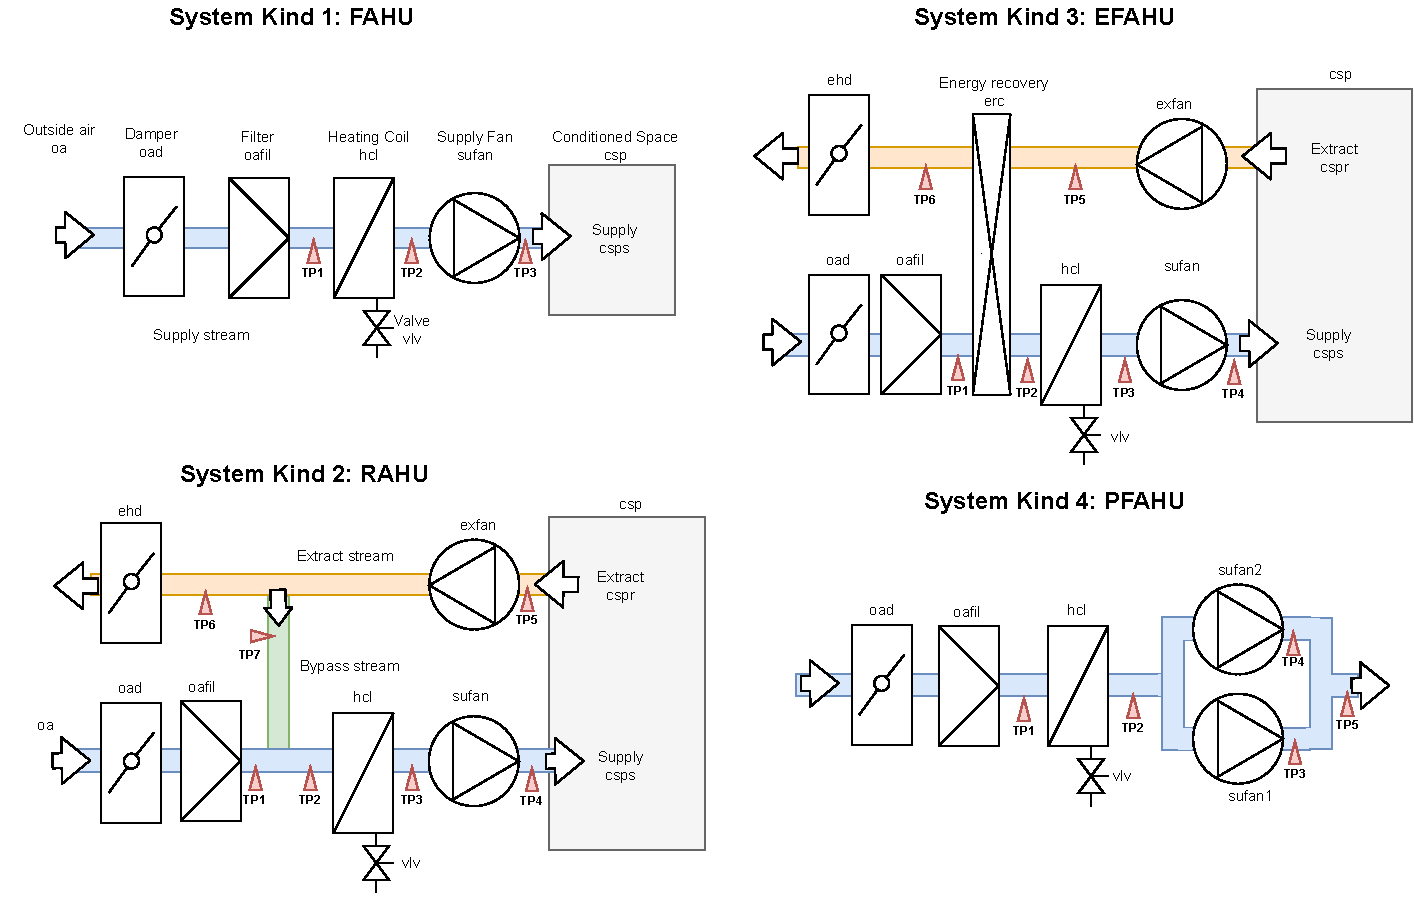
\includegraphics[width=0.78\linewidth]{figures/e_four_system_kinds.pdf}
\caption{The four system kinds identified for our evaluation. The labels on different components (like \textit{oad} or \textit{sufan}) are referred to in our results. The red triangles represent the test points identified in our evaluation.}
\label{fig:four-kinds-of-systems}
\end{figure*}

\begin{enumerate}
    \item SK1: Fresh-air AHU (FAHU). Topologically and process-wise, this represents a simple \emph{sequence of components and their physical mechanisms} in a single stream. 
    %The FAHU includes components that act both passively and actively on the process. Its heating coil component participates in two streams: the air-flow and the hot-water circulation.
    
    \item SK2: Recirculation AHU (RAHU). In addition to the features of a FAHU, a RAHU also has the merging and splitting of air streams. This hence \emph{extends the simple sequence} of components to a situation where components in different streams influence each-other.
    
    \item SK3: Energy-recovery AHU (ERAHU). In this case, an energy recovery component (heat exchanger) influences two process streams by transferring energy from one to another.
    This represents systems where an individual component manages flows of physical stuff (and, hence, dependencies) across different streams: Other than in the RAHU where the recirculated air stream enters the supply-side components directly, the ERAHU only transfers heat (and not air mass) between the two streams.
    
    \item SK4: Parallel-Fan AHU (PFAHU): This case introduces the parallel operation of two components (fans) which separate from a stream and later rejoin.
    This represents systems that feature parallel mechanisms that are stereotypically equivalent and feed jointly into a downstream component.
 
\end{enumerate}

Though these SKs are based on different configurations of AHUs, the process topology kinds they represent are also seen in other systems such as in chiller and boiler plants.

We defined two test cases to evaluate if topological descriptions where components are associated to stereotypes of their process mechanisms can be used to infer 1. the process dependencies between the components and 2. the effect of a component on a process variable observed at a given position in the stream.
We now describe the two test cases and the results in further detail.

\textbf{Test Case 1:} Given two components whose connection is described using a generic \textit{feeds} relation (such as \texttt{brick:feeds}), can our approach identify the \textit{physical process relationship} between them?
%For example, in the AHU, both filter and the valve are in \texttt{feeds} relationship to the heating coil.
%However, from a physical process standpoint, we need to know that the filter feeds air to the heating coil's air inlet and the valve feeds water (which then influences the air outlet temperature).

% A discussion such as for UC4 is missing here.

\textbf{Results:} Table~\ref{tab:uc3-results} summarizes the results for each pair connected components in each of the SKs.
For each of the connections, our approach helps to identify which process variables are affected on the upstream and downstream sides.
%
A HVAC domain expert examined the results and confirmed that the inferences were correct and no connection or associated effects were missing.

%=========================================================================
\begin{table*}[]
\begin{tabular}{|lll|lll|lll|lll|}
\hline
\multicolumn{3}{|c|}{\textbf{SK1}}                                                                                                                                                                                                                                                                                                              & \multicolumn{3}{c|}{\textbf{SK2}}                                                                                                                                                                                           & \multicolumn{3}{c|}{\textbf{SK3}}                                                                                                                                                                                                                                                  & \multicolumn{3}{c|}{\textbf{SK4}}                                                                                                                                                                                                                                                         \\ \hline
\multicolumn{1}{|l|}{\textbf{Connection}}                                                                                                             & \multicolumn{1}{l|}{\textbf{DSE}}                                                                     & \textbf{USE}                                                                    & \multicolumn{1}{l|}{\textbf{Connection}}                                                   & \multicolumn{1}{l|}{\textbf{DSE}}                                        & \textbf{USE}                                        & \multicolumn{1}{l|}{\textbf{Connection}}                                                                             & \multicolumn{1}{l|}{\textbf{DSE}}                                                       & \textbf{USE}                                                      & \multicolumn{1}{l|}{\textbf{Connection}}                                                                                     & \multicolumn{1}{l|}{\textbf{DSE}}                                                      & \textbf{USE}                                                      \\ \hline
\multicolumn{1}{|l|}{\begin{tabular}[c]{@{}l@{}}\texttt{oa} $\rightarrow$ \texttt{oadmp}\\ \texttt{oadmp} $\rightarrow$ \texttt{oafil}\\ \texttt{oafil} $\rightarrow$ \texttt{hcl}\\ \texttt{hcl} $\rightarrow$ \texttt{sufan}\\ \texttt{vlv} $\rightarrow$ \texttt{hcl}\\ \texttt{sufan} $\rightarrow$ \texttt{cspc}\end{tabular}} & \multicolumn{1}{l|}{\begin{tabular}[c]{@{}l@{}}none\\ flow\\ none\\ none\\ air T\\ flow\end{tabular}} & \begin{tabular}[c]{@{}l@{}}flow\\ none\\ none\\ flow\\ none\\ none\end{tabular} & \multicolumn{1}{l|}{\begin{tabular}[c]{@{}l@{}}exfan $\rightarrow$ hcl\\ exfan $\rightarrow$ ehdmp\end{tabular}} & \multicolumn{1}{l|}{\begin{tabular}[c]{@{}l@{}}flow\\ flow\end{tabular}} & \begin{tabular}[c]{@{}l@{}}none\\ flow\end{tabular} & \multicolumn{1}{l|}{\begin{tabular}[c]{@{}l@{}}exfan $\rightarrow$ erc\\ erc $\rightarrow$ ehdmp\\ oafil $\rightarrow$ erc\\ erc $\rightarrow$ hcl\end{tabular}} & \multicolumn{1}{l|}{\begin{tabular}[c]{@{}l@{}}flow\\ none\\ none\\ air T\end{tabular}} & \begin{tabular}[c]{@{}l@{}}none\\ none\\ none\\ none\end{tabular} & \multicolumn{1}{l|}{\begin{tabular}[c]{@{}l@{}}hcl $\rightarrow$ sufan1\\ hcl $\rightarrow$ sufan2\\ sufan1 $\rightarrow$ cspc\\ sufan2 $\rightarrow$ cspc\end{tabular}} & \multicolumn{1}{l|}{\begin{tabular}[c]{@{}l@{}}none\\ none\\ flow\\ flow\end{tabular}} & \begin{tabular}[c]{@{}l@{}}flow\\ flow\\ none\\ none\end{tabular} \\ \hline
\end{tabular}
\caption{Interconnection of components identified by HVAC domain expert and the downstream effects (DSE) and upstream effects (USE) they have on each other in terms of process variables they influence.}
\label{tab:uc3-results}

\end{table*}
%=========================================================================


\textbf{Test Case 2:} Find component(s) of a system which play a role in modulating a process variable observed at specified test points (TPs) in the process (e.g., ``Which components influence the supply temperature observed at the outlet of the heating coil?''). 

This test case is motivated from the use case of system diagnostics where a maintenance engineer attempts to identify components whose operation is likely to influence the process variable under question (see~\cite{arroyo2014integrating} for further details).
%
%Since we treat actuators as instances of \texttt{elem:Component} which have physical relations to other components, this UC also addresses determining actuators which eventually influence the physical process (e.g., mechanical force \textit{flows} from a valve actuator to a valve spindle, which eventually affects the fluid flow rate).
%
To aid the evaluation, our approach permits the definition of TPs at various locations in each of the SKs chosen for evaluation (see TP markers in Figure~\ref{fig:four-kinds-of-systems}).
%A TP is defined in terms of stream, process position, and stuff with respect to a component. For example air temperature in the supply stream at the outlet of the heating coil.
The TPs were chosen based on key process positions which are relevant for an AFDD use case~\cite{house2001expert}.
%In the system model, we represented the outside air (oa) and the conditioned space (csp) with variables that represent their state (temperature).
We asked a HVAC domain expert to list all components both upstream and downstream of the TPs which would influence temperature and air flow rate at each TP.
%
We then formulated SPARQL queries to automatically find instances of \texttt{elem:Components} that influence the temperature and air flow at each TP, and applied these queries to each of the four AHU configurations SK1-SK4.

\textbf{Results:}
%Table~\ref{tab:uc4-results} lists the components (identified by an HVAC expert) which influence temperature and flow at various TPs in the SKs.
Our proposed automatic approach achieved 100\% matching accuracy of influencing components in SK1 and SK3. 
At all TPs in these system kinds, our approach correctly identified the chain of dependencies between the components. For example, in TP3 in SK1, the dependencies for air flow are \texttt{sufan} and \texttt{oad}, and the dependencies for air temperature are \texttt{oa}, \texttt{oad}, \texttt{hcl}, \texttt{vlv}, and \texttt{sufan}.
Our approach performs equally well for SK3 because the energy transfer between two streams (supply and extract) is captured in the mechanism of the energy recovery component (\texttt{erc}), and therefore the flow of air in the streams are independent.

However, in SK2, our approach fails to correctly identify the influencing components at TP2, i.e., at one of the seven TPs; and in SK4, it fails with respect to two TPs -- for all these errors, our approach underreported influencing components, i.e., while its precision remained at 100\%, its recall dropped to 20\% for TP2 in SK2 and to 66\%/66\% for TP3/TP4 in SK4.

Regarding SK2, our approach correctly identified that at all TPs flow is influenced by \texttt{oad}, \texttt{sufan}, \texttt{exfan}, and \texttt{ehd}. However, at TP2, our approach identifies only the outdoor air (\texttt{oa}) temperature as the variable that influences temperature at TP2 while an expert identifies five additional factors: \texttt{cspr}, \texttt{exfan}, \texttt{sufan}, \texttt{ehd}, and \texttt{oad}; these factors determine how much air from the bypass will mix with outside air, and thereby influence the temperature at TP2.
%
The reason for this underreporting of dependencies in our approach is that it is missing a mechanism to model mixing physical stuff from two streams.
%footnote{For the conceptually similar setup in SK3, our system is able to correctly identify all factors because, here, the energy recovery component (\texttt{erc}) makes the energy (but not mass flow) transfer explicit in our model.}
This problem could be remedied in our HVAC stereotypes ontology by modeling \emph{conditioned space} as a stereotypical component with thermal (e.g., for heat gain) and hydrodynamic (e.g., for air flow) physical mechanisms; however, for our evaluation we chose to use a system that is modeled \emph{exclusively} based on an already available ontology -- in this case, Brick.
An important learning in this regard is that entities that may not \emph{directly} appear as components in a system topology (such as splits or joins in ducts, etc.) may play an important role in physical processes -- these should, hence, be added to ontologies such as Brick.

With respect to TP3 and TP4 in SK4, our approach of chaining variable dependencies in upstream and downstream directions does not handle a case where operation of one component affects the IV of another component in a \emph{parallel} stream.
Concretely, the expert identified that operation of \texttt{sufan1} will affect the inlet pressure of \texttt{sufan2} (and vice-versa), and hence the flow rate at both, TP3 and TP4, are dependent on \emph{both} fans.
This issue could be remedied in the same way as for SK2 -- that is, by modeling the splitting and joining of streams as explicit components.
%This can be addressed by integrating knowledge that permits us to express general laws of physics that are valid for a system as a whole -- in this case, conservation of mass and energy.
%We propose to accomplish this not by resorting to mathematical equations but by formulating the laws using a rule language such as SWRL~\footnote{\url{https://www.w3.org/Submission/SWRL/}}.


%===================================================================================================


\section{Conclusions and Future Work}

%Significant things to report:
%- The idea / concept of stereotypes
%- The ontology and SPARQL queries to implement this, together with specific stereotypes for HVAC
%- Application to office building
%- The proof that the stereotypes are covering HVAC: An openly available ontology for HVAC is Brick. They can nicely model real-life systems and the Brick classes for HVAC power 98\% of all components. Ganesh's Siemens Ontology does a bit better. Ganesh says that Brick:HU and Brick:Chiller are not components but they are subsystems because these employ connected chains of mechanisms. So from Brick, Ganesh has identified those concepts that actually are components (and not sub-systems), i.e. those that contain only a single physical mechanism. Ganesh has mapped those 19 components to the underlying (11) physical mechanism stereotypes. This makes Ganesh's account of physical mechanism stereotypes covering with respect to HVAC. 
%- A pilot verification of the mechanism stereotypes: Ganesh has verified with a colleague that the knowledge captured by the mechanism stereotypes and the way that this is related to component kinds is correct.

Our approach introduces a novel method of ontology-guided modeling of stereotypical behavior of components that are commonly used in building systems.
We have shown that with this approach we can create stereotypes corresponding to HVAC component classes in Brick, which can then be associated to actual instances of components in the system.
Further, we validated using real-life engineering information that the stereotypes capture a high-level abstraction of the underlying physical mechanisms which is sufficient to correlate possible actions on the component to the observable effects.
This knowledge about the local behavior of each component in a system then helps us infer their cumulative effect on the physical process conducted by the system.
We evaluated our approach on systems deployed in real life which displayed largely positive results; however, in process topologies which contain mixing mass flow streams, we identified the need to extend our system with a way to model physical laws that apply to the system in its entirety.
%
Our work seeks to bring together research on semantic modeling of system design and physical processes so that it opens up the possibility for software programs such as for AFDD and plausibility checking to use machine-understandable knowledge to reason about behavior of a system. For higher-fidelity system simulation, our approach is compatible with the attaching of complete simulation models to building automation components.


%Move this to future work.
%In addition to describing physical mechanisms in terms of relationships to variables, we propose a way to describe the \textit{tendencies} (also called \textit{trends} or \textit{qualitative proportionality})\cite{top1991computational} they exhibit, i.e. the direction in which the dependent variable responds to change in the independent variable.
%To model this, we introduce the relationships \texttt{elem:attenuates} and \texttt{elem:boosts} as sub-properties of \texttt{elem:modulates} to express if the modulation of the independent variable will cause the dependent variable to be actively decreased or increased.


%The relationships described above can be expressed as:
%\begin{align*}
%    \forall m,v_d,v_m\ (ProcessMechanism(m) \land hasDependentVariable(m,v_d) \\
%    \land hasManipulatedVariable(v_m) \rightarrow \exists v_m,v_d\ (modulates(v_m,v_d)))
%\end{align*}

%As we shall see later, our approach in distinguishing the \texttt{elem:ManipulatedProcessVariable} helps reason about the effect of component actions in a process chain.

%Additionally,  the affliation of a ProcessVariable to physical stuff can be used along  with basic laws in physics such as laws conservation of mass and energy to infer relationship between variables at the boundary of the mechanism.
%\begin{align*}
%    \forall m,v_d,v_i\ (ProcessMechanism(m) \land hasDependentVariable(m,v_d) \\
%    \land hasIndependentVariable(v_i) \land hasSubstance(v_i, s)\\
%    \rightarrow \exists v_d\ (hasSubstance(v_d,v_i)))
%\end{align*}

\bibliographystyle{ACM-Reference-Format}
\bibliography{references}

\end{document}
\endinput
%%
%% End of file `sample-sigconf.tex'.
